\section{ÔN TẬP CHƯƠNG 4}
\subsection{Câu trắc nghiệm nhiều phương án lựa chọn}
\textit{Thí sinh trả lời từ câu 1 đến câu 18. Mỗi câu thí sinh chọn một phương án}
\setcounter{ex}{0}
\Opensolutionfile{ans}[ans/VN12-Y24-PH-SYL-030-TN]
% ===================================================================
\begin{ex}
	Trong hạt nhân nguyên tử $\ce{^{210}_{84}Po}$ có
	\choice
	{84 proton và 210 neutron}
	{126 proton và 84 neutron}
	{\True 84 proton và 126 neutron}
	{210 proton và 84 neutron}
	\loigiai{}
\end{ex}
% ===================================================================
\begin{ex}
	Năng lượng liên kết riêng của một hạt nhân
	\choice
	{có thể âm hoặc dương}
	{\True càng lớn thì hạt nhân càng bền}
	{càng nhỏ thì hạt nhân càng bền}
	{có thể triệt tiêu, đối với một số hạt nhân đặc biệt}
	\loigiai{}
\end{ex}
% ===================================================================
\begin{ex}
	Cho phản ứng hạt nhân: $\ce{^{210}_{84}Po}\longrightarrow\ce{X}+\ce{^{206}_{82}Pb}$. Hạt $\ce{X}$ là
	\choice
	{$\ce{^1_1H}$}
	{$\ce{^3_2He}$}
	{\True $\ce{^4_2He}$}
	{$\ce{^3_1H}$}
	\loigiai{}
\end{ex}
% ===================================================================
\begin{ex}
	Cho phản ứng hạt nhân: $\ce{^3_1T}+\ce{^2_1D}\longrightarrow\alpha+\ce{n}$. Biết $m_{\ce{T}}=\SI{3.01605}{u}$; $m_{\ce{D}}=\SI{2.01411}{u}$; $m_{\alpha}=\SI{4.00260}{u}$; $m_{\ce{n}}=\SI{1.00867}{u}$; $\SI{1}{u}=\SI{931}{\mega\electronvolt/c^2}$. Năng lượng tỏa ra khi một hạt $\alpha$ được hình thành là
	\choice
	{\True $\SI{17.6}{\mega\electronvolt}$}
	{$\SI{23.4}{\mega\electronvolt}$}
	{$\SI{11.04}{\mega\electronvolt}$}
	{$\SI{16.7}{\mega\electronvolt}$}
	\loigiai{}
\end{ex}
% ===================================================================
\begin{ex}
	Biết số Avogadro $N_A=\SI{6.02E23}{\mole^{-1}}$ và khối lượng của hạt nhân bằng số khối của nó. Số proton có trong $\SI{0.27}{\gram}\ \ce{^{27}_{13}Al}$ là
	\choice
	{$\SI{6.826E22}{}$}
	{$\SI{8.826E22}{}$}
	{$\SI{9.826E22}{}$}
	{\True $\SI{7.826E22}{}$}
	\loigiai{}
\end{ex}
% ===================================================================
\begin{ex}
	Đại lượng nào sau đây đặc trưng cho mức độ bền vững của hạt nhân?
	\choice
	{Năng lượng nghỉ}
	{Độ hụt khối}
	{Năng lượng liên kết}
	{\True Năng lượng liên kết riêng}
	\loigiai{}
\end{ex}
% ===================================================================
\begin{ex}
	Phát biểu nào sau đây là \textbf{sai} khi nói về lực hạt nhân?	
	\choice
	{\True Lực hạt nhân có bản chất là lực điện}
	{Lực hạt nhân là lực hút}
	{Lực hạt nhân chỉ có tác dụng khi khoảng cách giữa hai nucleon bằng hoặc nhỏ hơn kích thước hạt nhân}
	{Lực hạt nhân là loại lực mạnh nhất trong các loại lực đã biết hiện nay}
	\loigiai{}
\end{ex}
% ===================================================================
\begin{ex}
	Phát biểu nào sau đây là \textbf{sai} khi nói về hiện tượng phóng xạ?
	\choice
	{Trong phóng xạ $\alpha$, hạt nhân con có số neutron nhỏ hơn số neutron của hạt nhân mẹ}
	{Trong phóng xạ $\beta^{-}$, hạt nhân mẹ và hạt nhân con có số khối bằng nhau, số proton khác nhau}
	{\True Trong phóng xạ $\beta$, có sự bảo toàn điện tích nên số proton được bảo toàn}
	{Trong phóng xạ $\beta^+$, hạt nhân mẹ và hạt nhân con có số khối bằng nhau, số neutron khác nhau}
	\loigiai{}
\end{ex}
% ===================================================================
\begin{ex}
\immini{Trong đồ thị ở hình dưới
	\choice
{$N_0$ là số hạt nhân lúc ban đầu $\left(t=0\right)$ của khối chất phóng xạ và $N$ là số hạt nhân của khối chất phóng xạ đã phân rã tính đến thời điểm $t$}
{\True $N_0$ là số hạt nhân lúc ban đầu của khối chất phóng xạ và $N$ là số hạt nhân còn lại của khối chất phóng xạ tính đến thời điểm $t$}
{$N_0$ là khối lượng ban đầu của khối chất phóng xạ và $N$ là khối lượng của các hạt nhân đã phân rã của khối chất phóng xạ tính đến thời điểm $t$}
{$N_0$ là khối lượng ban đầu của khối chất phóng xạ và $N$ là khối lượng còn lại của khối chất phóng xạ tính đến thời điểm $t$}
}
{\begin{tikzpicture}  
		\begin{axis}[  ultra thick,scale=0.75,
			xmin=0,  
			xmax=4,  
			xtick={0,1,...,3},
			ytick={0,1,2,4,8},
			minor x tick num=1,
			minor y tick num=1,
			yticklabels={0,$N_0/8$, $N_0/4$,$N_0/2$,$N_0$},
			ymin=0,  
			ymax=9, 
			samples=300,
			axis lines=center, 
			grid style={step=1, line width =0.4pt, color=gray!30!white},
			grid=both, %giới hạn ô lưới
			major grid style={line width=0.8pt,gray!60!white},
			xlabel=$\xsi{t}{\left(\si{\hour}\right)}$, 		ylabel=$\xsi{N}{\left(\text{hạt}\right)}{}$,
			every axis y label/.style={at=(current axis.above origin),anchor=south},  
			every axis x label/.style={at=(current axis.right of origin),anchor=west},  ]
			\addplot [ultra thick, blue, smooth, domain=0:4] {8*2^(-x)};  
		\end{axis}  
\end{tikzpicture}}
	\loigiai{}
\end{ex}
% ===================================================================
\begin{ex}
	Coi hạt nhân nguyên tử như một quả cầu bán kính $R=\xsi{1,2\cdot10^{-15}\cdot A^{\frac{1}{3}}}{\left(\meter\right)}$ với $A$ là số khối. Bán kính của hạt nhân $\ce{^{27}_{13}Al}$ có giá trị bằng
	\choice
	{$\SI{0.36E-12}{\meter}$}
	{$\SI{3.6E-12}{\meter}$}
	{$\SI{0.36E-15}{\meter}$}
	{\True $\SI{3.6E-15}{\meter}$}
	\loigiai{}
\end{ex}
% ===================================================================
\begin{ex}
	Một chất phóng xạ có chu kì bán rã là $\SI{3.8}{\text{ngày}}$. Sau thời gian $\SI{11.4}{\text{ngày}}$ thì độ phóng xạ của lượng chất phóng xạ còn lại bằng bao nhiêu phần trăm so với độ phóng xạ của lượng chất  phóng xạ ban đầu?
	\choice
	{$\SI{25}{\percent}$}
	{$\SI{75}{\percent}$}
	{\True $\SI{12.5}{\percent}$}
	{$\SI{87,5}{\percent}$}
	\loigiai{
		$H=H_02^{-\frac{t}{T}}$.
	}
\end{ex}

% ===================================================================
\begin{ex}
	Một chất phóng xạ mà hạt nhân của nó phát ra một hạt $\alpha$ rồi biến đổi thành hạt nhân $\ce{X}$ bền vững. Trong 1 phút đầu tiên có $n_1$ hạt $\alpha$ bắn ra và sau đó $\SI{24}{\hour}$ thì trong 1 phút có $n_2=0,3294n_1$ hạt $\alpha$ bắn ra. Chu kì bán rã của chất đó xấp xỉ bằng
	\choice
	{\True 15 giờ}
	{138 ngày}
	{3,8 ngày}
	{50 giờ}
	\loigiai{
		$$H_2=H_1\cdot2^{-\frac{t}{T}}\Rightarrow \frac{H_2}{H_1}=\dfrac{n_2}{n_1}=2^{-\frac{t}{T}}$$
		$$\Leftrightarrow \log_2 0,3294 =\frac{\left(\SI{24}{\hour}\right)}{T}\Rightarrow T\approx\SI{15}{\hour}.$$
	}
\end{ex}
% ===================================================================
\begin{ex}
	Cho ba hạt nhân X, Y và Z có số nucleon tương ứng là $A_{\ce{X}}$, $A_{\ce{Y}}$, $A_{\ce{Z}}$ với $A_{\ce{X}}=2A_{\ce{Y}}=0,5A_{\ce{Z}}$. Biết năng lượng liên kết của từng hạt nhân tương ứng là $\Delta E_{\ce{X}}$, $\Delta E_{\ce{Y}}$, $\Delta E_{\ce{Z}}$ với $\Delta E_{\ce{Z}}<\Delta E_{\ce{X}}<\Delta E_{\ce{Y}}$. Sắp xếp các hạt nhân này theo thứ tự tính bền vững giảm dần là
	\choice
	{X, Y, Z}
	{Z, X, Y}
	{\True Y, X, Z}
	{Y, Z, X}
	\loigiai{}
\end{ex}
% ===================================================================
\begin{ex}
	Tại một thời điểm, số hạt nhân trong mẫu phóng xạ còn lại bằng $\SI{25}{\percent}$ so với số hạt nhân ở thời điểm ban đầu $\left(t=0\right)$. Sau thời điểm đó $\SI{10}{\second}$, số hạt nhân chưa bị phân rã còn lại bằng $\SI{12.5}{\percent}$ so với số hạt nhân ở thời điểm ban đầu $\left(t=0\right)$. Chu kì bán rã của chất phóng xạ đó là
	\choice
	{\True $\SI{10}{\second}$}
	{$\SI{20}{\second}$}
	{$\SI{25}{\second}$}
	{$\SI{12.5}{\second}$}
	\loigiai{
		Trong khoảng thời gian $\SI{10}{\second}$ số hạt nhân còn lại giảm từ $0,25N_0$ xuống còn $0,125N_0$ (giảm 1 nửa). Nên chu kì bán rã của chất phóng xạ trên $T=\SI{10}{\second}$.
	}
\end{ex}
% ===================================================================
\begin{ex}
	Chất phóng xạ polonium $\ce{^{210}_{84}Po}$ phát ra tia $\alpha$ và biến đổi thành chì $\ce{^{206}_{82}Pb}$. Gọi chu kì bán rã của polonium là $T$. Ban đầu $\left(t=0\right)$ có một mẫu nguyên chất. Trong khoảng thời gian từ $t=0$ đến $t=2T$ có $\SI{63}{\milli\gram}$ polonium trong mẫu bị phân rã. Lấy khối lượng nguyên tử tính theo đơn vị $\si{u}$ bằng số khối của hạt nhân nguyên tử đó. Trong khoảng thời gian từ $t=2T$ đến $t=3T$, lượng $\ce{^{206}_{82}Pb}$ được tạo thành trong mẫu có khối lượng là
	\choice
	{$\SI{72.1}{\milli\gram}$}
	{$\SI{5.25}{\milli\gram}$}
	{$\SI{73.5}{\milli\gram}$}
	{\True $\SI{10.3}{\milli\gram}$}
	\loigiai{
		Từ $t_0=0$ đến $t_1=2T$ số hạt $\ce{Po}$ bị phân rã:
		$$\Delta N=\dfrac{\Delta m}{M}N_A=\dfrac{\SI{63E-3}{\gram}}{\SI{210}{\gram/\mole}}\cdot\left(\SI{6.022E23}{\mole^{-1}}\right).$$
		Mà $\Delta N=N_0\left(1-2^{-\frac{t_1}{T}}\right)=\dfrac{3}{4}N_0\Rightarrow N_0=\SI{2.4E20}{}.$\\
		Từ $t_1=2T$ đến $t_2=3T$ thì số hạt $\ce{Po}$ bị phân rã là 
		$$\Delta N'=N_0\left(2^{-\frac{t_1}{T}}-2^{-\frac{t_2}{T}}\right)=\dfrac{1}{8}N_0=\SI{0.3E20}{}$$
		Khối lượng chì tạo thành:
		$$m_{\ce{Pb}}=\dfrac{\Delta N'}{N_A}\cdot M_{\ce{Pb}}\approx\SI{10.26}{\milli\gram}.$$
	}
\end{ex}
% ===================================================================
\begin{ex}
	Trong phản ứng tổng hợp helium: $\ce{^7_3Li}+\ce{^1_1H}\longrightarrow2 \ce{^4_2He}+\SI{15.1}{\mega\electronvolt}$, nếu tổng hợp helium từ $\SI{1}{\gram}$ litium thì năng lượng tỏa ra có thể đun sôi bao nhiêu $\si{\kilo\gram}$ nước có nhiệt độ ban đầu là $\SI{0}{\celsius}$? Lấy nhiệt dung riêng của nước $c=\SI{4200}{\joule/\left(\kilogram\cdot\kelvin\right)}$.	
	\choice
	{\True $\SI{4.95E5}{\kilogram}$}
	{$\SI{1.95E5}{\kilogram}$}
	{$\SI{3.95E5}{\kilogram}$}
	{$\SI{2.95E5}{\kilogram}$}
	\loigiai{
		Dựa vào phương trình phản ứng ta thấy, 1 hạt $\ce{Li}$ tổng hợp ra $\ce{He}$ tỏa năng lượng $\SI{15.1}{\mega\electronvolt}$.\\
		Trong $\SI{1}{\gram}\ \ce{Li}$ có $N=\SI{8.604E22}{\text{hạt nhân}}$.\\
		Năng lượng tỏa ra khi tổng hợp hết $\SI{1}{\gram}\ \ce{Li}$ là:
		$$\Delta E=15,1\cdot\SI{8.604E22}{}\cdot\SI{1.6E-13}{}=\SI{2.078E11}{\joule}.$$
		Lượng nước có thể được đun sôi:
		$$m=\dfrac{\Delta E}{c\left(100-0\right)}\approx\SI{4.95E5}{\kilo\gram}.$$
	}
\end{ex}
% ===================================================================
\begin{ex}
	Dùng proton có động năng $K_p=\SI{5.45}{\mega\electronvolt}$ bắn phá hạt nhân $\ce{^9_4Be}$ đứng yên sinh ra hạt $\alpha$ và $\ce{X}$. Giả sử phản ứng không kèm theo bức xạ gamma, cho $\SI{1}{u}=\SI{931}{\mega\electronvolt/c^2}$. Biết động năng của hạt $\alpha$ là $K_\alpha=\SI{4}{\mega\electronvolt}$, hướng của proton bay tới và hướng của hạt $\alpha$ vuông góc với nhau. Xem khối lượng các hạt bằng số khối. Tốc độ của hạt $\ce{X}$ xấp xỉ bằng
	\choice
	{\True $\SI{10.7E6}{\meter/\second}$}
	{$\SI{2.7E8}{\meter/\second}$}
	{$\SI{1.7E8}{\meter/\second}$}
	{$\SI{0.1E6}{\meter/\second}$}
	\loigiai{
		Bảo toàn động lượng:
		$$\vec{p}_p=\vec{p}_{\alpha}+\vec{p}_{\ce{X}}$$
		$$\Rightarrow \vec{p}_{\ce{X}}=\vec{p}_p-\vec{p}_{\alpha}$$
		Vì $\vec{p}_p\bot\vec{p}_{\alpha}$ nên:
		\begin{eqnarray*}
			&&p^2_{\ce{X}}=p^2_p+p^2_{\alpha}\\
			&\Rightarrow& m_{\ce{X}}K_{\ce{X}}=m_{\alpha}K_{\alpha}+m_pK_p\\
			&\Rightarrow& K_{\ce{X}}=\SI{3,575}{\mega\electronvolt}.
		\end{eqnarray*}
		Tốc độ của hạt $\ce{X}$ xấp xỉ:
		$$v_{\ce{X}}=\sqrt{\dfrac{2K_{\ce{X}}}{m_{\ce{X}}}}=\sqrt{\dfrac{2\cdot\left(\SI{3.575}{\mega\electronvolt}\right)}{6\cdot\left(\SI{931}{\mega\electronvolt/c^2}\right)}}=0,036c\approx\SI{10.7E6}{\meter/\second}.$$
	}
\end{ex}
% ===================================================================
\begin{ex}
	Một proton vận tốc $v$ bắn vào hạt nhân litium $\left(\ce{^7_3Li}\right)$ đứng yên. Phản ứng tạo ra hai hạt nhân $\ce{X}$ giống hệt nhau với vận tốc có độ lớn bằng $v'$ và cùng hợp với phương tới của proton một góc $\SI{60}{\degree}$, $m_{\ce{X}}$ là khối lượng nghỉ của hạt $\ce{X}$. Giá trị của $v'$ là
	\choice
	{\True $\dfrac{m_pv}{m_{\ce{X}}}$}
	{$\dfrac{m_{\ce{X}}v\sqrt{3}}{m_p}$}
	{$\dfrac{m_{\ce{X}}v}{m_p}$}
	{$\dfrac{m_pv\sqrt{3}}{m_{\ce{X}}}$}
	\loigiai{
		Tam giác vector động lượng được tạo bởi ba cạnh $\vec{p}_{\ce{X}}; \vec{p}_{\ce{X}}; \vec{p}_{p}$ là tam giác đều nên:
		$$p_{\ce{X}}=p_p\Leftrightarrow m_{\ce{X}}v'=m_pv\Rightarrow v'=\dfrac{m_pv}{m_{\ce{X}}}.$$
	}
\end{ex}
\Closesolutionfile{ans}
\subsection{Câu trắc nghiệm đúng/sai}
\textit{Thí sinh trả lời từ câu 1 đến câu 4. Trong mỗi ý \textbf{a)}, \textbf{b}, \textbf{c)}, \textbf{d)} ở mỗi câu, thí sinh chọn đúng hoặc sai}
\setcounter{ex}{0}
\Opensolutionfile{ans}[ans/VN12-Y24-PH-SYL-030-TF]
% ===================================================================
\begin{ex}
	Hạt nhân $\ce{^7_3Li}$ có khối lượng $\SI{7.0144}{u}$. Cho khối lượng của proton và neutron lần lượt là $\SI{1.0073}{u}$ và $\SI{1.0087}{u}$, $\SI{1}{u}=\SI{931.5}{\mega\electronvolt/c^2}$.
	\choiceTF[t]
	{Hạt nhân $\ce{^7_3Li}$ có 3 proton và 4 nucleon}
	{\True Độ hụt khối của hạt nhân $\ce{^7_3Li}$ là $\Delta m=\SI{0.0423}{u}$}
	{\True Năng lượng liên kết của hạt nhân $\ce{^7_3Li}$ là $E_{\text{lk}}=\SI{39.4}{\mega\electronvolt}$}
	{Năng lượng liên kết riêng của hạt nhân $\ce{^7_3Li}$ là $\SI{13.13}{\mega\electronvolt/\text{nucleon}}$}
	\loigiai{}
\end{ex}
% ===================================================================
\begin{ex}
	Cho phản ứng hạt nhân $\ce{^{37}_{17}Cl}+\ce{X}\longrightarrow\ce{^{37}_{18}Ar}+\ce{n}$. Cho $m_{\ce{Cl}}=\SI{36.9566}{u}$; $m_{\ce{Ar}}=\SI{36.9569}{u}$; $m_{\ce{X}}=\SI{1.0073}{u}$; $m_{\ce{n}}=\SI{1.0087}{u}$; $\SI{1}{u}=\SI{931}{\mega\electronvolt/c^2}$.\\
	Xét tính đúng/sai của các phát biểu dưới đây: 
	\choiceTF[t]
	{\True Hạt nhân $\ce{X}$ là $\ce{^1_1H}$ (hydrogen)}
	{Phản ứng này là phản ứng tỏa năng lượng}
	{Năng lượng tỏa ra của phản ứng là $\SI{1.58}{\mega\electronvolt}$}
	{\True Đồng vị $\ce{Ar}$ trong phản ứng có số khối là 37}
	\loigiai{}
\end{ex}
% ===================================================================
\begin{ex}
	\immini{Chiếu xạ thực phẩm có thể tiêu diệt vi khuẩn và côn trùng làm cho thực phẩm có thời hạn sử dụng lâu hơn. Ví dụ, thời gian sử dụng của dâu tây có thể tăng lên từ 4 ngày thành 20 ngày bằng cách chiếu tia $\gamma$ vào quả dâu tây sau khi hái. Không chỉ vi khuẩn mà côn trùng và trứng côn trùng cũng bị tiêu diệt khi bị chiếu xạ. Hình bên mô tả các hộp thực phẩm được vận chuyển nhờ băng truyền qua máy chiếu xạ. }
	{\includegraphics[scale=0.12]{figs/VN12-Y24-PH-SYL-033P-1}}
	Nguồn phóng xạ của máy là cobalt $\ce{^{60}_{27}Co}$, phát ra bức xạ $\beta$ và $\gamma$. Cho biết chu kì bán rã của $\ce{^{60}_{27}Co}$ là 5,72 năm.
	Hình dưới đây là đồ thị tỉ lệ phần trăm cường độ bức xạ $\gamma$ truyền qua một lớp trái cây có độ dày nhất định.
	\begin{center}
		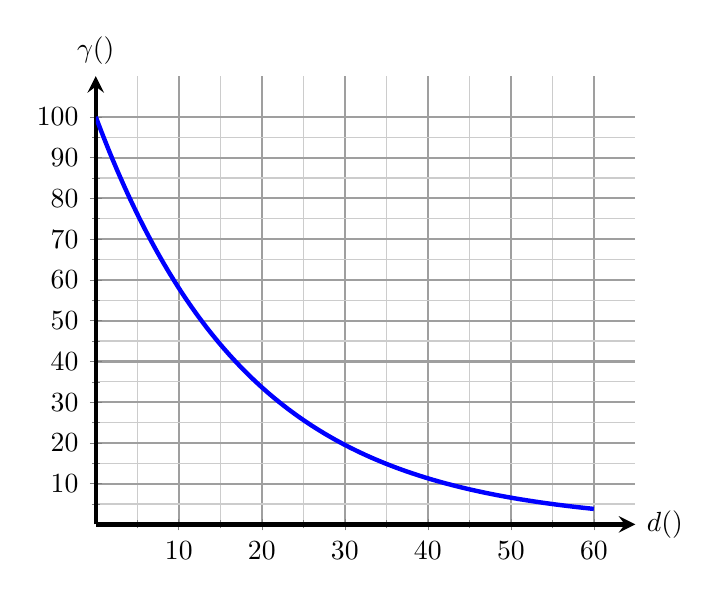
\begin{tikzpicture}  
			\begin{axis}[  ultra thick,
				xmin=0,  
				xmax=65,  
				xtick={0,10,...,60},
				ytick={0,10,...,100},
				minor x tick num=1,
				minor y tick num=1,
				ymin=0,  
				ymax=110, 
				samples=300,
				axis lines=center, 
				grid style={step=1, line width =0.4pt, color=gray!40!white},
				grid=both, %giới hạn ô lưới
				major grid style={line width=0.8pt,gray!75!white},
				xlabel=$\xsi{d}{\left(\si{\centi\meter}\right)}$, 		ylabel=$\xsi{\gamma}{\left(\si{\percent}\right)}$,
				every axis y label/.style={at=(current axis.above origin),anchor=south},  
				every axis x label/.style={at=(current axis.right of origin),anchor=west},  ]  
				\addplot [ultra thick, blue, smooth, domain=0:60] {100*2^(-x/12.726)}; 
			\end{axis}  
		\end{tikzpicture}
	\end{center}
	\choiceTF[t]
	{\True Phương trình phân rã của $\ce{^{60}_{27}Co}$ là: 	$\ce{^{60}_{27}Co}\xrightarrow{\beta^-}\ce{^{60}_{28}Ni}+\ce{^0_{-1}e}+\gamma.$
	}
	{\True Bức xạ $\beta$ mà $\ce{^{60}_{27}Co}$ phát ra hầu như không góp phần tiêu diệt vi khuẩn và côn trùng trong trái cây}
	{Từ đồ thị trên, xác định được độ dày của trái cây để cường độ bức xạ $\gamma$ giảm $\SI{50}{\percent}$ là $\SI{15}{\centi\meter}$}
	{Theo thời gian, độ phóng xạ của nguồn $\ce{^{60}_{27}Co}$ giảm dần.  Nếu nguồn phóng xạ vẫn có thể sử dụng được cho đến khi độ  phóng xạ của nó giảm xuống còn $\SI{12.5}{\percent}$ giá trị ban đầu thì sau 30 năm sẽ phải thay nguồn phóng xạ $\ce{^{60}_{27}Co}$}
	\loigiai{}
\end{ex}
% ===================================================================
\begin{ex}
	Hình bên là đồ thị mô tả sự phụ thuộc số hạt của hai mẫu chất phóng xạ $\ce{X}$ và $\ce{Y}$ theo thời gian $t$ ($N_{\ce{X}}$ là đường đứt nét; $N_{\ce{Y}}$ là đường liền nét).
	\begin{center}
		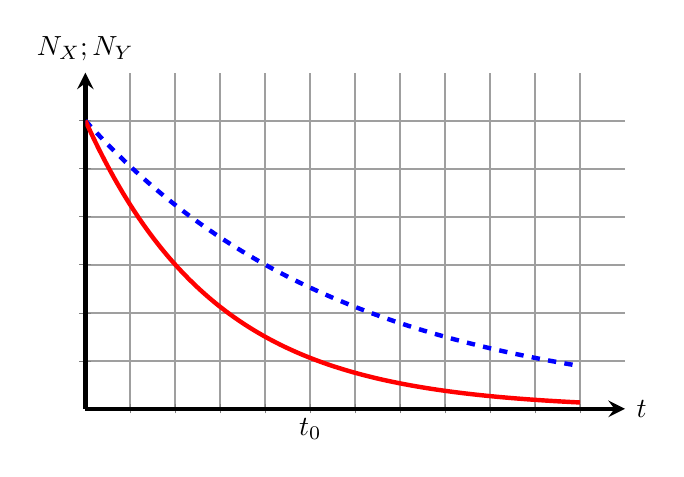
\begin{tikzpicture}  
			\begin{axis}[  ultra thick,yscale=0.75,
				xmin=0,  
				xmax=12,  
				xtick={0,1,...,11},
				ytick={0,1,...,6},
				ymin=0,  
				ymax=7, 
				minor x tick num=0,
				minor y tick num=0,
				samples=300,
				yticklabels=\empty,
				xticklabels=\empty,
				axis lines=center, 
				grid style={step=1, line width =0.4pt, color=gray!40!white},
				grid=both, %giới hạn ô lưới
				major grid style={line width=0.8pt,gray!75!white},
				xlabel=$t$, 		ylabel=$N_{\ce{X}}; N_{\ce{Y}}$,
				every axis y label/.style={at=(current axis.above origin),anchor=south},  
				every axis x label/.style={at=(current axis.right of origin),anchor=west},  ]
				\coordinate (t0) at (axis cs: 5,0);
				\addplot [ultra thick, blue, dashed, smooth, domain=0:11] {6*2^(-x/4)};  
				\addplot [ultra thick, red, smooth, domain=0:11] {6*2^(-x/2)}; 
			\end{axis}  
			\node[below] at(t0) {$t_0$};
		\end{tikzpicture}
	\end{center}
	\choiceTF[t]
	{\True Chu kì bán rã của $\ce{X}$ lớn hơn chu kì bán rã của $\ce{Y}$}
	{Tại thời điểm ban đầu, độ phóng xạ của hai mẫu chất bằng nhau}
	{\True Tại thời điểm $t_0$, số hạt $\ce{Y}$ còn lại xấp xỉ $\SI{17.7}{\percent}$ số hạt ban đầu}
	{Hằng số phóng xạ của $\ce{X}$ gấp 3 hằng số phóng xạ của $\ce{Y}$}
	\loigiai{
		\begin{itemchoice}
			\itemch Đúng. Chu kì bán rã của $\ce{X}$ gấp đôi chu kì bán rã của $\ce{Y}$.
			\itemch Sai. Số hạt ban đầu bằng nhau nhưng hằng số phóng xạ khác nhau nên độ phóng xạ ban đầu khác nhau.
			\itemch Đúng. Coi như chu kì bán rã của $\ce{Y}$ là $T_{\ce{Y}}=2$ và $t_0=5\Rightarrow$ số hạt $\ce{Y}$ còn lại là $N_{\ce{Y}}=N_0\cdot2^{-\frac{5}{2}}$.
			\itemch Sai. Hằng số phóng xạ của $\ce{X}$ bằng một nửa hằng số phóng xạ của $\ce{Y}$.
		\end{itemchoice}
	}
\end{ex}
\Closesolutionfile{ans}
\subsection{Câu trắc nghiệm trả lời ngắn} \textit{Thí sinh trả lời từ câu 1 đến câu 6}
\setcounter{ex}{0}
\Opensolutionfile{ans}[ans/VN12-Y24-PH-SYL-030-TL]
% ===============================================================
\begin{ex}
	Biết số Avogadro $N_A=\SI{6.02E23}{\mole^{-1}}$. Trong $\SI{59.50}{\gram}\ \ce{^{238}_{92}U}$ có số neutron xấp xỉ là bao nhiêu \textit{(Kết quả tính theo bội số $10^{25}$ và làm tròn đến 3 CSCN)}?
	\shortans[oly]{2,20}
	\loigiai{
		Số neutron trong mỗi hạt nhân $\ce{^{238}_{92}U}$ là $n=238-92=146$.\\
		Số neutron có trong $\SI{59.50}{\gram}\ \ce{^{238}_{92}U}$:
		$$N=\dfrac{m}{M}N_A\cdot n=\SI{2.20E25}{}.$$
	}
\end{ex}
% ===============================================================
\begin{ex}
	Để tách các hạt nhân $\ce{^4_2He}$ có trong $\SI{1}{\gram}\ \ce{^4_2He}$ thành các proton và neutron tự do thì cần năng lượng bao nhiêu \textit{(tính theo đơn vị $\SI{e11}{\joule}$ và làm tròn đến hàng phần trăm)}? Cho biết $m_{\ce{He}}=\SI{4.0015}{u}$; $m_p=\SI{1.0073}{u}$; $m_n=\SI{1.0087}{u}$; $\SI{1}{u}=\SI{931.5}{\mega\electronvolt/c^2}=\SI{1.66055E-27}{\kilogram}$ và $\SI{1}{\electronvolt}=\SI{1.6E-19}{\joule}$.
	\shortans[oly]{6,84}
	\loigiai{
		Năng lượng liên kết của $\ce{He}$: $E_{\text{lk}}=\SI{28.41}{\mega\electronvolt}$.\\
		Số hạt $\ce{He}$ có trong $\SI{1}{\gram}$: $N=\dfrac{\SI{E-3}{\gram}}{4,0015\cdot\left(\SI{1.66055E-27}{\kilogram}\right)}=\SI{1.5E23}{\text{hạt}}$.\\
		Năng lượng cần thiết: 
		$$E=N\cdot E_{\text{lk}}=\SI{4.28E24}{\mega\electronvolt}=\SI{6.84E11}{\joule}.$$
	}
\end{ex}
% ===============================================================
\begin{ex}
	\immini{
	Một mẫu chất phóng xạ nguyên chất có hằng số phóng xạ $\lambda$, số hạt ban đầu là $N_0$, số hạt tại thời điểm $t$ là $N$. Hình bên mô tả đồ thị của $\ln N$ theo $t$. Xác định độ phóng xạ ban đầu của mẫu chất \textit{(Kết quả tính theo đơn vị $\si{\second^{-1}}$ và làm tròn đến 3 CSCN)}.
	}
	{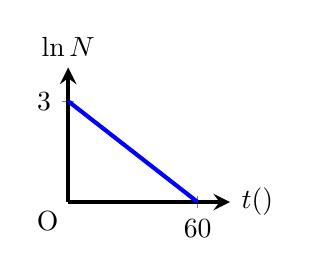
\begin{tikzpicture}  
			\begin{axis}[  ultra thick,scale=0.3,
				xmin=0,  
				xmax=75,  
				xtick={0,60},
				ytick={0,3},
				ymin=0,  
				ymax=4, 
				samples=300,
				axis lines=center, 
				xlabel=$\xsi{t}{\left(\si{\second}\right)}$, 		ylabel=$\ln N$,
				every axis y label/.style={at=(current axis.above origin),anchor=south},  
				every axis x label/.style={at=(current axis.right of origin),anchor=west},  ]
				\draw[blue, line width=1.5pt] (axis cs:0,3)--(axis cs: 60,0); 
			\end{axis} 
			\node[below left] at(0,0) {O}; 
	\end{tikzpicture}}
	\shortans[oly]{1,00}
	\loigiai{
		Từ $N=N_0e^{-\lambda t}\Rightarrow \ln N=\ln N_0-\lambda t$.\\
		Ta có:
		$$\begin{cases}
			\text{Tại}\ t=\SI{0}{\second}; \ln N=3\\
			\text{Tại}\ t=\SI{60}{\second}; \ln N=0\\
		\end{cases}\Rightarrow\begin{cases}
			\ln N_0=3\\
			\ln N_0-60\lambda=0
		\end{cases}\Rightarrow\begin{cases}
			N_0=e^3\\
			\lambda=\SI{0.05}{\second^{-1}}
		\end{cases}.$$
		Độ phóng xạ ban đầu của mẫu chất:
		$$H_0=\lambda N_0\approx\SI{1.0043}{\second^{-1}}.$$
	}
\end{ex}
% ===============================================================
\begin{ex}
	Các vụ nổ hạt nhân cũng được sử dụng cho mục đích hòa bình (PNEs). Năm 1966, một vụ nổ hạt nhân đã được kích nổ tại mỏ khí đốt Urtabulak ở miền Nam Uzbekistan để dập tắt đám cháy từ một giếng khí đốt. Người ta khoan 2 lỗ vào lòng đất cách giếng khoảng $\SI{35}{\meter}$ với độ sâu $\SI{1500}{\meter}$. Các chất nổ hạt nhân với đương lượng $\SI{30}{\text{kiloton}}$ được đưa vào các lỗ khoan và cho kích nổ. Ngay sau vụ nổ, ngọn lửa đã tắt và cái giếng đã bị bịt kín. Tính khối lượng $\ce{^{235}U}$ trong vụ nổ trên. Nếu năng lượng của vụ nổ trên là do sự phân hạch của $\ce{^{235}U}$ và mỗi phân hạch tỏa năng lượng $\SI{200}{\mega\electronvolt}$, biết $\SI{1}{\text{kiloton}}$ là đương lượng nổ với năng lượng tương ứng $\SI{4.186E12}{\joule}$. \textit{(Kết quả tính theo đơn vị gram và làm tròn đến 4 CSCN)}.
	\shortans[oly]{1532}
	\loigiai{
		Năng lượng của một phân hạch $\ce{^{235}U}$ là: $\Delta E=200\cdot\SI{1.6E-13}{}=\SI{3.2E-11}{\joule}.$\\
		Năng lượng của vụ nổ: $E=30\cdot\SI{4.186E12}{}=\SI{1.2558E14}{\joule}$.\\
		Khối lượng $\ce{^{235}U}$ cần dùng là: 
		$$m=\dfrac{E}{\Delta E}\cdot\dfrac{1}{N_A}\cdot235=\SI{1532}{\gram}.$$	
	}
\end{ex}
% ===============================================================
\begin{ex}
	Ban đầu $\left(t=0\right)$ có một mẫu chất phóng xạ $\ce{X}$ nguyên chất, ở thời điểm $t_1$ mẫu chất phóng xạ $\ce{X}$ còn lại $\SI{20}{\percent}$ hạt nhân chưa bị phân rã. Đến thời điểm $t_2=t_1+\SI{100}{\second}$, số hạt nhân $\ce{X}$ chưa bị phân rã chỉ còn $\SI{5}{\percent}$ so với số hạt nhân ban đầu. Chu kì bán rã của $\ce{X}$ là bao nhiêu giây?	
	\shortans[oly]{ 50}
	\loigiai{
		Theo đề bài ta có:
		$$\begin{cases}
			N_{t1}=\SI{20}{\percent}N_0\\
			N_{t2}=\SI{5}{\percent}N_0
		\end{cases}\Rightarrow \begin{cases}
			2^{-\frac{t_1}{T}}=0,2\\
			2^{-\frac{t_2}{T}}=0,05
		\end{cases}\Rightarrow 2^{\frac{t_2-t_1}{T}}=4\Rightarrow 2^{\frac{100}{T}}=4\Rightarrow T=\SI{50}{\second}.$$
	}
\end{ex}
% ===============================================================
\begin{ex}
	Dùng hạt $\alpha$ có động năng $\SI{5.00}{\mega\electronvolt}$ bắn vào hạt nhân $\ce{^{14}_7N}$ đứng yên gây ra phản ứng: $\ce{^4_2He}+\ce{^{14}_7N}\longrightarrow\ce{X}+\ce{^1_1H}$. Phản ứng này thu năng lượng $\SI{1.21}{\mega\electronvolt}$ và không kèm theo bức xạ gamma. Lấy khối lượng các hạt nhân tính theo đơn vị $\si{u}$ bằng số khối của chúng. Khi hạt nhân $\ce{X}$ bay ra theo hướng lệch với hướng chuyển động của hạt $\alpha$ một góc lớn nhất thì động năng của hạt $\ce{X}$ có giá trị là bao nhiêu \textit{(Kết quả tính theo đơn vị $\si{\mega\electronvolt}$ và làm tròn đến 2 CSCN)}?
	\shortans[oly]{0,90 }
	\loigiai{
		Bảo toàn năng lượng toàn phần:
		$$\Delta E=K_{\ce{X}}+K_{\ce{H}}-K_{\alpha}\Rightarrow K_{\ce{X}}+K_{\ce{H}}=\SI{3.79}{\mega\electronvolt}.$$
		Bảo toàn động lượng:
		$$\vec{p}_{\alpha}=\vec{p}_{\ce{X}}+\vec{p}_{\ce{H}}$$
		$$\Rightarrow \vec{p}_{\ce{H}}=\vec{p}_{\alpha}-\vec{p}_{\ce{X}}$$
		Bình phương 2 vế phương trình trên ta thu được:
		\begin{eqnarray*}
			&&p^2_{\ce{H}}=p^2_{\alpha}+p^2_{\ce{X}}-2p_{\alpha}p_{\ce{X}}\cos\beta\\
			&\Leftrightarrow& m_{\ce{H}}K_{\ce{H}}=m_{\alpha}K_{\alpha}+m_{\ce{X}}K_{\ce{X}}-2\sqrt{m_{\alpha}m_{\ce{X}}K_{\alpha}K_{\ce{X}}}\cos\beta\\
			&\Leftrightarrow& 3,79-K_{\ce{X}}=20+17K_{\ce{X}}-4\sqrt{85}\cdot\sqrt{K_{\ce{X}}}\cos\beta\\
			&\Rightarrow& 4\sqrt{85}\cos\beta=\dfrac{16,21}{\sqrt{K_{\ce{X}}}}+18\sqrt{K_{\ce{X}}}
		\end{eqnarray*}
		Áp dụng bất đẳng thức Cauchy:
		$$4\sqrt{85}\cos\beta\ge 2\sqrt{16,21\cdot18}=34,16\Rightarrow \beta\le\SI{22.12}{\degree} $$
		Dấu "=" của bất đẳng thức xảy ra khi: 
		$$\dfrac{16,21}{\sqrt{K_{\ce{X}}}}=18\sqrt{K_{\ce{X}}}\Rightarrow K_{\ce{X}}=\SI{0.90}{\mega\electronvolt}.$$
	}
\end{ex}
\Closesolutionfile{ans}
